\documentclass[tikz,border=10pt]{standalone}
\usepackage{amsmath}
\begin{document}
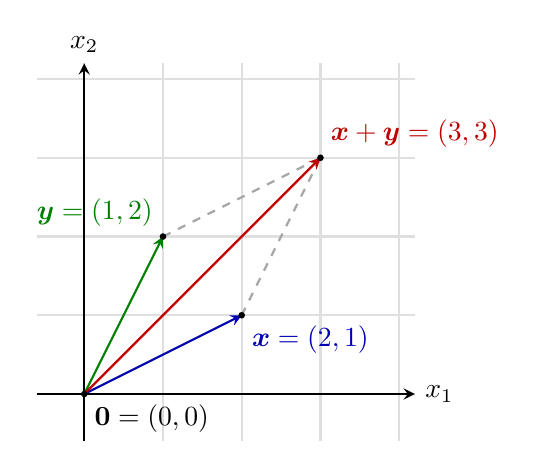
\begin{tikzpicture}[scale=1, >=stealth, line width=0.8pt]
  % Cuadrícula
  \draw[gray!25, step=1cm] (-0.6,-0.6) grid (4.2,4.2);

  % Ejes
  \draw[->] (-0.6,0) -- (4.2,0) node[right] {$x_1$};
  \draw[->] (0,-0.6) -- (0,4.2) node[above] {$x_2$};

  % Vectores
  \draw[->, thick, blue!70!black] (0,0) -- (2,1) node[below right] {$\boldsymbol{x}=(2,1)$};
  \draw[->, thick, green!50!black] (0,0) -- (1,2) node[above left] {$\boldsymbol{y}=(1,2)$};

  % Paralelogramo / traslación
  \draw[dashed, gray!70] (2,1) -- (3,3);
  \draw[dashed, gray!70] (1,2) -- (3,3);

  % Vector suma
  \draw[->, thick, red!75!black] (0,0) -- (3,3) node[above right] {$\boldsymbol{x}+\boldsymbol{y}=(3,3)$};

  % Puntos
  \fill (0,0) circle (1.2pt) node[below right] {$\boldsymbol{0}=(0,0)$};
  \fill (2,1) circle (1.2pt);
  \fill (1,2) circle (1.2pt);
  \fill (3,3) circle (1.2pt);
\end{tikzpicture}
\end{document}
